\begin{frame}[t]
	\frametitle{Headline - Very Serious}
	One item
	\begin{itemize}
		\item Here it is.
	\end{itemize}
	\pause
	\vspace{0.5cm}
	Two items
	\begin{itemize}
		\item Item 1. \pause
		\item Item 2.
		\item Item 3.
	\end{itemize}
	\note[item] {Not actually serious}
	\note[item] {
	Venn Diagrams
	\\
		\begin{figure}[h]
			\centering
			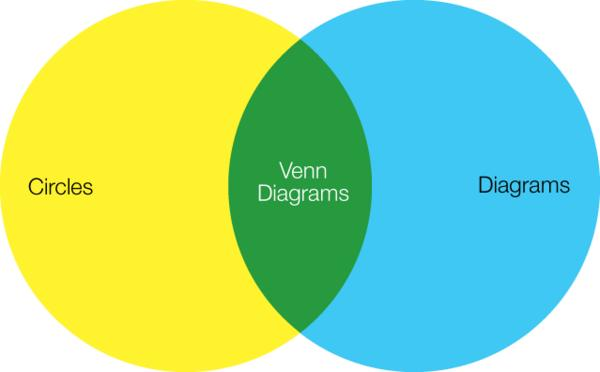
\includegraphics[height=\textheight/2]{img/venndiagram.jpeg}
			\label{fig:venndiagram-meta}
		\end{figure}
	}
\end{frame}

\begin{frame}[t]
	\frametitle{Range query searching}
	\begin{block}{S1. [Search subtrees.]}
		 Check each entry $E$ to determine whether the MBR overlaps $q$.
		 For all overlapping entries, invoke \emph{Search} on the tree whose
		 root is pointed to by $E.p$
	\end{block}

	\begin{block}{S2. [Search leaf node.]}
		Check all entries $E$ to determine whether the MBR overlaps $q$.
		If so, $E$ is a qualifying record
	\end{block}
\end{frame}
